\section{Subespacios vectoriales, bases y coordenadas}

\begin{itemize}[label=\color{red}\textbullet, leftmargin=*]
	\item \color{lightblue}Definición (Subespacio vectorial)
\end{itemize}

Un subespacio vectorial de $\K^n$ es un subconjunto $W$ de $\K^n$ que cumple:
\begin{enumerate}[label=\color{lightblue}\arabic*)]
	\item Si $w,w'\in W\longrightarrow w+w'\in W$
	\item Si $w\in W$ y $\alpha\in\K\longrightarrow\alpha w\in W$
\end{enumerate}
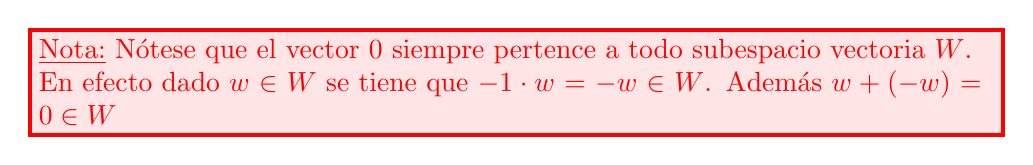
\begin{tikzpicture}
	\node[red,draw=red,fill=red!10, line width=1.5,text width=\textwidth] {\underline{Nota:} Nótese que el vector 0 siempre pertence a todo subespacio vectoria $W$. En efecto dado $w\in W$ se tiene que $-1\cdot w=-w\in W$. Además $w+(-w)=0\in W$};
\end{tikzpicture}

\Ej

Sean $A\in M_{m\times n}(\K)$ y $W$ el conjunto de soluciones del sistema $Ax=0$. Entonces, $w$ es un subespacio vectorial. En efecto: si $w,w^\perp\in W$, entonces $Aw=0,Aw'=0$. Por tanto, $A(w+w')=Aw+Aw'=0+0=0$, lo que implica que $w+w'\in W$.

Si $w\in W$ y $\alpha\in\K$, entonces $Aw=0$ y $A(\alpha w)=\alpha Aw=0$. Por tanto, $aw\in W$.

A este subespacio se le llama núcleo de $A$ y se denota $\mathrm{nuc}(A)$.

\bu{Ejemplo 1}

Sea $W=\K^n$. Entonces los vectores \[ B=\{e_1=(1,0,\dots,0),e_2=(0,1,0,\dots,0)\},\dots,e_n=(0,\dots,0,1) \] son una base de $W$. En efecto:
\begin{enumerate}[label=\color{lightblue}\arabic*)]
	\item $B$ es un conjunto generador ya que si $v=(v_1,\dots,v_n)\in\K^n$, entonces \begin{align*}
		v&=v_1e_1+v_2e_2+\cdots+v_ne_n\\
		&=v_1(1,0,\dots,0)+v_2(0,1,0,\dots,0)+\cdots+v_n(0,\dots,0,1)
	\end{align*}
	\item $B$ es linealmente independiente:
	
	$\sum\alpha_ie_i=0\longleftrightarrow\alpha_1(1,0,\dots,0)+\alpha_2(0,1,0,\dots,0)+\cdots+a_n(0,\dots,0,1)=(0,\dots,0)$
	
	$(\alpha_1,\alpha_2,\dots,\alpha_n)=(0,\dots,0)$
\end{enumerate}

\bu{Ejemplo 2}

Sean $A=\begin{bmatrix}
	1 & -1 & 1\\
	1 & 1 & 1
\end{bmatrix}$ y $W=\mathrm{nuc}(A)$.

Vamos a obtener una base de $W$.\[ Ax=0\longleftrightarrow\begin{bmatrix}
	1 & -1 & 1\\
	1 & 1 & 1
\end{bmatrix}\cdot\begin{bmatrix}
x_1\\
x_2\\
x_3
\end{bmatrix}=\begin{bmatrix}
x_1-x_2+x_3\\
x_1+x_2+x_3
\end{bmatrix}=\begin{bmatrix}
0\\
0
\end{bmatrix} \]$\begin{rcases}
x_1-x_2+x_3=0\\
x_1+x_2+x_3=0
\end{rcases}\quad\mathrm{rg}(A)=2<3=$nº de incógnitas

Desde un punto de vista computacional interesa disponer de bases ortonormales. El Algoritmo de Gram-Schmidt proporciona un método sistemático para construir una base ortonormal a partir de otra dada.
\begin{itemize}[label=\color{red}\textbullet, leftmargin=*]
	\item \color{lightblue}Teorema (Algoritmo de Gram-Schmidt)
\end{itemize}
Sea $\{v_1,v_2,\dots,v_m\}$ un conjunto de vectores lineales independiente de $\R^n$. Entonces, existe un conjunto ortonormal $\{u_1,u_2,\dots,u_m\}$ de modo que \[ <v_1,v_2,\dots,v_m>=<u_1,u_2,\dots,u_m> \]
\begin{itemize}[label=\color{red}\textbullet, leftmargin=*]
	\item \color{lightblue}Demostración
\end{itemize}
\begin{enumerate}[label=\color{lightblue}\arabic*)]
	\item Sea $v_1'=v_1$
	\item $v_2'=v_2+\alpha v_1$. Imponemos 
	
	$0=v_1'\cdot v_2'=v_1\cdot v_2+\alpha v_1\cdot v_1'=v_1'\cdot v_2+\alpha\|v_1'\|^2\longrightarrow\alpha=-\dfrac{v_1\cdot v_2}{\|v_1\|^2}\longrightarrow v_2'=v_2-\dfrac{v_1\cdot v_2}{\|v_1\|^2}v_1$
	
	obviamente $<v_1,v_2>=<v_1',v_2'>$
	\item $v_3'=v_3+\alpha v_2'+\beta v_1'$. Imponemos
	
	$0=v_3'\cdot v_2'=v_3\cdot v_2'+\alpha v_2'v_2'+\tozero{\beta v_1'v_2'}\longrightarrow\alpha=-\dfrac{v_3\cdot v_2'}{\|v_2'\|^2}$
	
	$0=v_3'\cdot v_1'=v_3\cdot v_1'+\tozero{\alpha v_2'\cdot v_1'}+\beta v_1'\cdot v_1'\longrightarrow\beta=-\dfrac{v_3\cdot v_1'}{v_1'\cdot v_1'}=-\dfrac{(0,1,1)-(1,1,0)}{2}=-\dfrac{1}{2}$
	
	$v_3'=(0,1,1)+\dfrac{1}{3}\left(\dfrac{1}{2},-\dfrac{1}{2},1\right)-\dfrac{1}{2}(1,1,0)$
	
	Finalmente: \[ u_1=\dfrac{v_1'}{\|v_1\|},\quad u_2=\dfrac{v_2'}{\|v_2'\|},\quad u_3=\dfrac{v_3'}{\|v_3'\|} \]
\end{enumerate}
\subsection{Suma de subespacios vectoriales}
\begin{itemize}[label=\color{red}\textbullet, leftmargin=*]
	\item \color{lightblue}Definición (Suma de subespacios)
\end{itemize}
Sean $U,V\subset\K^n$ dos subespacios vectoriales. Se llama suma de los subespacios $u$ y $v$, denotado, \[ U+V=\{w=u+v,u\in U,v\in W\} \]obviamente, $U+V$ es un subespacio vectorial.

Además, si $U=<u_1,\dots,u_r>,V=<v_1,\dots,v_s>$ entonces \[ U+V=<u_1,\dots,u_r,v_1,\dots,v_s>.\]

\begin{itemize}[label=\color{red}\textbullet, leftmargin=*]
	\item \color{lightblue}Proposición
\end{itemize}
La suma $U+V$ es directa si y sólo si $U\cap V=\{0\}$. En este caso, cada vector $w\in U\oplus V$ se escribe de forma única como $w=u+v,u\in U,v\in W$.
\subsection{Ortogonal a un subespacio}
\begin{itemize}[label=\color{red}\textbullet, leftmargin=*]
	\item \color{lightblue}Definición
\end{itemize}
Dado un subespacio vectorial $U\subset\R^n$, se define su subespacio ortogonal como \[ U^\perp=\{v\in\R^n:u\cdot v=0\:\forall u\in U\} \]
\begin{itemize}[label=\color{red}\textbullet, leftmargin=*]
	\item \color{lightblue}Proposición
\end{itemize}
Sea $U\subset\R^n$ un subespacio vectorial. Entonces \[ U\oplus U^\perp=\R^n\]
\begin{itemize}[label=\color{red}\textbullet, leftmargin=*]
	\item \color{lightblue}Demostración
\end{itemize}
Es fácil ver que $u^\perp$ es un subespacio vectorial. Además, si $u\in U\cap U^\perp$ entonces $u\cdot u=0\longrightarrow u=0$.

Sea $B$ una base ortogonal de $U$ y la ampliamos a una base ortogonal $B\cup B'$ de $\R^n$. Entonces \[ \R^n=<B>\oplus <B'>\subseteq U\oplus U^\perp\subset\R^n \]
\subsection{Subespacios asociados a una matriz. Rango}\begin{itemize}[label=\color{red}\textbullet, leftmargin=*]
	\item \color{lightblue}Definición
\end{itemize}
Dada $A\in M_{m\times n}$, definimos los siguientes subespacios, llamados fundamentales, de $A$:
\begin{enumerate}[label=\color{lightblue}\arabic*)]
	\item $\mathrm{Col}(A)=$ subespacio generado por las columnas de $A$.
	\item $\fil(A)=$ subespacio generado por las filas de $A$.
	\item $\nuc(A)=$ subespacio generado por las soluciones del sistema $Ax=0$. (núcleo por la derecha)
	\item $\nuc(A^\intercal)=$ subespacio generado por las soluciones del sistema $A^\intercal x=0$, que también se escribe como $x^\intercal A=0$.
\end{enumerate}
\begin{itemize}[label=\color{red}\textbullet, leftmargin=*]
	\item \color{lightblue}Proposición
\end{itemize}
\[ \rg(A)=\dimf(A)=\dimc(A). \]
\begin{itemize}[label=\color{red}\textbullet, leftmargin=*]
	\item \color{lightblue}Demostración
\end{itemize}
\begin{enumerate}[label=\color{lightblue}\arabic*)]
	\item Veamos que si $P$ es invertible, entonces \[ \dimc(PA)=\dimc(A) \] Sea $r=\dimc(A)$ y $\{u_1,u_2,\dots,u_r\}$ una base de $\col(A)$.
	
	Entonces $\{Pu_1,\dots,Pu_r\}$ son linealmente independientes. Por tanto, $r\le\dimc(PA)$.
	
	Recíprocamente, si $\{Pu_1,\dots,Pu_s\}$ es una base de $\col(PA)$ entonces $\{P^{-1}Pu_1,\dots,P^{-1}Pu_s\}$ son linealmente independientes. Por tanto, $s\le r$ y así $\dimc(A)=\dimc(PA)$.
	\item De igual modo se prueba que si $Q$ es invertible, entonces $\dimf(AQ)=\dimf(A)$.
	\item Consideremos la factorización $PAQ$ de $A$, es decir, \[ PAQ=\left(\begin{array}{c|c}
		Ir & 0\\ \hline
		0 & 0
	\end{array}\right) \]y recordemos que el rango es el número de pivotes no nulos.
	
	Por lo visto anteriormente se tiene el resultado.
\end{enumerate}
\begin{itemize}[label=\color{red}\textbullet, leftmargin=*]
	\item \color{lightblue}Teorema (Rank-nullity)
\end{itemize}
Sea $A\in M_{m\times n}(\K)$. Entonces \[ \bboxed{\rg(A)=\dimn(A)=n} \]

$\begin{vmatrix}
	2 & 1\\
	1 & 0
\end{vmatrix}\neq0,\qquad\begin{vmatrix}
2 & 2 & 1\\
1 & 1 & 0\\
1 & 1 & 1
\end{vmatrix}=0,\qquad\begin{vmatrix}
2 & 1 & 1\\
1 & 0 & 0\\
1 & 1 & 1
\end{vmatrix}=0$

Por tanto, $\rg(A)=2$

\subsection{Coordenadas respecto de una base}
Sean $W\subset\K^n$ un subespacio vectorial y $B=\{u_1,u_2,\dots,u_m\}$ una base de $W$.

Entonces, todo vector de $W$ se expresa de \lb{modo único} como combinación lineal de los vectores de $B$.

En efeto: sea $w\in W$ y supongamos que \[ w=\sum_{i=1}^{m}\alpha_iu_i=\sum_{i=1}^{m}\beta_1u_1. \]Entonces, \[ \sum_{i=1}^{m}(\alpha_i-\beta_i)u_i=0\xrightarrow[\begin{subarray}{c}
		\{u_i\}\\
		\text{lin. ind.}
\end{subarray}]{}\alpha_i-\beta_i=0 \]
\begin{itemize}[label=\color{red}\textbullet, leftmargin=*]
	\item \color{lightblue}Definición
\end{itemize}
Sea $W$ un subespacio vectorial de $\K^n$ y $B=\{u_1,u_2,\dots,u_m\}$ una base de $W$.

Dado $w\in W$, se llaman \lb{coordenadas} de $w$ en la base $B$ a los únicos escalares $(x_1,x_2,\dots,x_m)\in\K^n$ tales que $w=x_1u_1+\cdots+x_mu_m$. Se denota: \[ [w]_B=(x_1,\dots,x_m) \]

\newpage

\begin{wrapfigure}[4]{r}{0.3\textwidth}
	\begin{tikzpicture}[scale=0.7]
		\draw (-2,0) -- (5,0);
		\draw (0,-4.2) -- (0,4);
		\draw[lightblue,-latex,line width=1.5] (0,0) -- (1,2) node[above right] {$v_1$};
		\draw[lightblue,-latex,line width=1.5] (0,0) -- (2,-1) node[below right] {$v_2$};
		\draw[blue,-latex,line width=1.5] (0,0) -- (1,-4) node[below right] {$v_1'$};
		\draw[blue,-latex,line width=1.5] (0,0) -- (0,-1) node[left] {$v_2'$};
		\draw[lightblue,dashed] (0,2) -- (1,2) -- (1,0);
		\draw[lightblue,dashed] (0,-1) -- (2,-1) -- (2,0);
		\draw[blue,dashed] (1,0) -- (1,-4) -- (0,-4);
		\draw[blue,dashed] (1,2) -- (3,1) node[right] {$v$} -- (2,-1) ;
		\foreach \x in {-1,...,3}{
		\draw (\x,0.1) -- (\x,-0.1);
		}
		\foreach \y in {-4,...,3}{
			\draw (0.1,\y) -- (-0.1,\y);
		}
	\end{tikzpicture}
\end{wrapfigure}

\Ej\\
$W=\R^2$

$B=\{v_1=(1,2),v_2=(2,-1)\}$\\
$B'=\{v_1'=(1,-3),v_2'=(0,1)\}$\\
Vamos a clauclar $M_{B\to B'}$

$v_1=(1,2)=a_{11}\cdot v_1'+a_{21}\cdot v_2'=a_{11}(1,-3)+a_{21}(0,-1)$\[ \begin{rcases}
	1=a_{11}\\
	2=-3a_{11}-a_{21}
\end{rcases}\begin{array}{l}
\\
\longrightarrow a_{21}=-3a_{11}-2=-5
\end{array} \]$v_2=(2,-1)=a_{12}\cdot v_1'+a_{22}\cdot v_2'=a_{12}(1,-3)+a_{22}(0,-1)$\[ \begin{array}{c}
\begin{cases}
2=a_{12}\\
-1=-3a_{12}-a_{22}
\end{cases}\begin{array}{l}
\\
\longrightarrow a_{22}=1-3a_{12}=-5
\end{array}\\
M_{B\to B'}=\begin{bmatrix}
		1 & 2\\
		-5 & -5
\end{bmatrix}
\end{array} \]
Sea ahora $[v]_B=(1,1)$, ¿$[v]_{B'}$?\begin{align*}
	[v]_{B'}&=M_{B\to B'}\cdot[v]_b\\
	&=\begin{bmatrix}
		1 & 2\\
		-5 & -5
	\end{bmatrix}_{2\times 2}\cdot\begin{bmatrix}
	\\
	1
	\end{bmatrix}_{2\times1}\\
	&=\begin{bmatrix}
		3\\
		10
	\end{bmatrix}
\end{align*}
\subsection{Coordenadas en bases ortonormales}
Supongamos que $B=\{u_1,\dots,u_m\}$ es una base ortonormal de $W$, es decir, \[ \begin{array}{l}
	u_i\cdot u_j=\delta_{ij}=\begin{cases}
		1 & \text{si }i=j\\
		0 & \text{si }i\neq0
	\end{cases}\text{ delta de Kronecker}\\
	\|u_i\|=1,\:1\le i\le m
\end{array} \]
Vamos a calcular la forma que tiene $[w]_B$, siendo $w\in W$. Se tiene: \[ w=\sum x_iu_i \]Por tanto: \[w\cdot u_j=\sum x_i\cdot u_i\cdot u_j=x_j \]es decir, \[ [w]_B=(w\cdot u_j) \]
Además, como \[\begin{aligned}
	w\cdot u_j&=\|w\|\cdot\|u_j\|\cos(w,u_j)\\
	&=\|w\|\cos(w,u_j)
\end{aligned}\] con lo que si $\|w\|=1\longrightarrow[w]_B=\underbrace{\left(\cos(w,u_j)\right)}_{\begin{subarray}{l}
	\text{cosenos directores}\\
	\text{del vector $w$}
	\end{subarray}}$

\begin{itemize}[label=\color{red}\textbullet, leftmargin=*]
	\item \color{lightblue}Resumen: \bu{Subespacios fudamentales de una matriz y resolución de sistemas lineales}
\end{itemize}

$A\in M_{m\times n}$
\begin{itemize}
	\item $\fil(A),\nuc(A)$ son subespacios vectoriales de $\R^n$
	\item $\fil(A)\perp\nuc(A)$
\end{itemize}

\[ Av=\left[\begin{array}{c}
	\text{fila }1\\
	\text{fila }2\\ \hdashline
	\text{fila }m\\
\end{array}\right]\qquad v=\left[\begin{array}{c}
\text{fila }1\cdot v\\
\text{fila }2\cdot v\\ \hdashline
\text{fila }m\cdot v
\end{array}\right]=0 \]
Por tanto, si $v\in\nuc(A)\longrightarrow v\perp$ todas las filas de $A$

$\begin{rcases}
	\rg(A)=\dimf(A)=r\\
	\rg(A)+\dimn(A)=n
\end{rcases}\longrightarrow\fil(A)\oplus\nuc(A)=\R^n$

\begin{center}
	
\includegraphics[width=\textwidth]{"Temas/Tema 4/resumen 4.drawio.png"}
\end{center}

\begin{itemize}
	\item $\col(A),\nuc(A^\intercal)$ son subespacios vectoriales de $\R^m$
	\item $\col(A)\perp\nuc(A^\intercal)$
\end{itemize}
\[ A^\intercal v=\left[\begin{array}{c}
	\text{Col }1^\intercal\\
	\text{Col }2^\intercal\\ \hdashline
	\text{Col }m^\intercal
\end{array}\right]\qquad v=\left[\begin{array}{c}
\text{Col }1^\intercal\cdot v\\
\text{Col }2^\intercal\cdot v\\ \hdashline
\text{Col }n^\intercal \cdot v
\end{array}\right]=0 \]
Por tanto, si $v\in\nuc(A^\intercal)\longrightarrow v\perp$ columnas de $A$

$\rg(A^\intercal)+\dimn(A^\intercal)=m\longrightarrow\col(A)\oplus\nuc(A^\intercal)$




